%%% HPBench system overview — COMPACT variant (reduced height).
%%% Drops per-panel pykeen/hpbench sublabels (colour + legend carry it),
%%% merges chips, thins the tasks band. Same content as hpbench_overview.tex.
\documentclass[tikz,border=0pt]{standalone}
\usepackage{amsmath,amssymb}
\usepackage[T1]{fontenc}
\usetikzlibrary{arrows.meta, positioning, shapes.misc, calc, backgrounds, fit}

% ── Colour palette (project-wide) ───────────────────────────────────────
\definecolor{varblue}{HTML}{3B82F6}
\definecolor{uriteal}{HTML}{0D9488}
\definecolor{wingreen}{HTML}{059669}
\definecolor{costamber}{HTML}{D97706}
\definecolor{edgegray}{HTML}{475569}
\definecolor{titledark}{HTML}{1E293B}
\definecolor{levelbox}{HTML}{94A3B8}
\definecolor{blankslate}{HTML}{64748B}
\definecolor{panelbg}{HTML}{F8FAFC}
\definecolor{querybg}{HTML}{F1F5F9}

\begin{document}
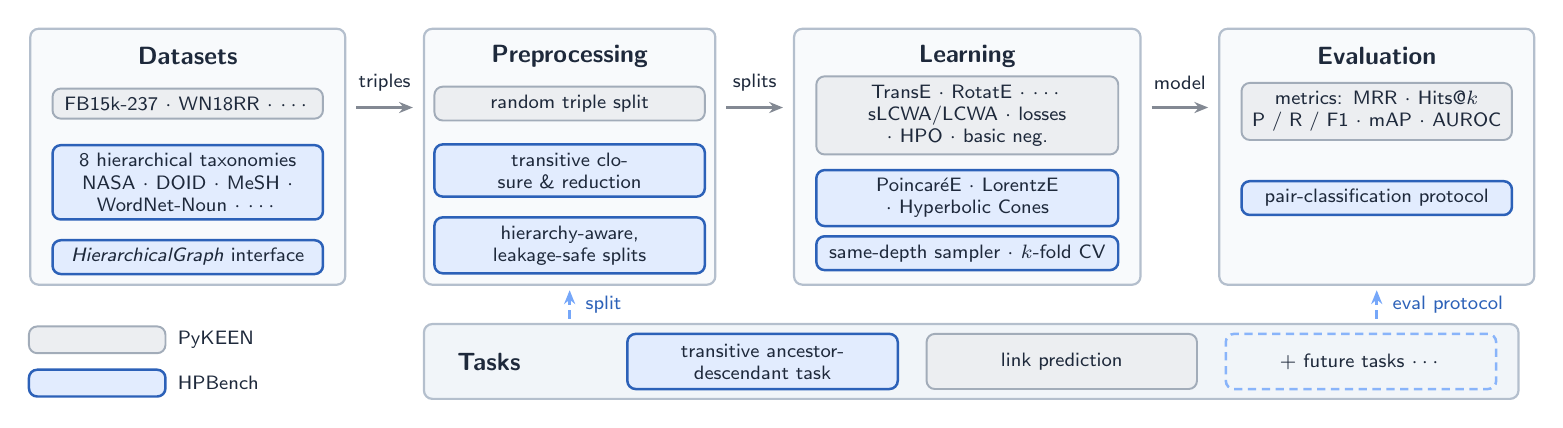
\begin{tikzpicture}[
    font=\sffamily,
    >={Stealth[length=5pt, width=4pt]},
    % ── shared styles ──
    sub label/.style={font=\scriptsize\sffamily, text=titledark},
    inner box/.style={draw=levelbox!70, line width=0.8pt, rounded corners=3pt,
        fill=panelbg},
    module title/.style={font=\small\sffamily\bfseries\scshape, text=titledark},
    pyk chip/.style={draw=blankslate!60, fill=blankslate!12, rounded corners=3pt,
        line width=0.7pt, font=\scriptsize\sffamily, text=titledark,
        align=center, inner ysep=3pt, text width=#1},
    hp chip/.style={draw=varblue!75!black, fill=varblue!15, rounded corners=3pt,
        line width=0.9pt, font=\scriptsize\sffamily, text=titledark,
        align=center, inner ysep=3pt, text width=#1},
    future chip/.style={draw=varblue!60, dash pattern=on 3pt off 2pt,
        rounded corners=3pt, line width=0.9pt, font=\scriptsize\sffamily,
        text=titledark, align=center, inner ysep=3pt, text width=#1},
    transition/.style={draw=titledark!55, line width=1.4pt, ->,
        shorten <=4pt, shorten >=4pt},
    configures/.style={->, draw=varblue!70, line width=0.9pt,
        dash pattern=on 3pt off 2pt, shorten <=2pt, shorten >=2pt},
    tlabel/.style={font=\scriptsize\sffamily, text=titledark, align=center},
]

% ══════════════════════════════════════════════════════════════════════
%  DIMENSIONS
% ══════════════════════════════════════════════════════════════════════
\def\panelT{0}    \def\panelB{-3.25}
\def\DL{0}    \def\DR{4.0}    \def\Dcx{2.0}    % Datasets
\def\PL{5.0}  \def\PR{8.7}    \def\Pcx{6.85}   % Preprocessing
\def\LL{9.7}  \def\LR{14.1}   \def\Lcx{11.9}   % Learning
\def\EL{15.1} \def\ER{19.1}   \def\Ecx{17.1}   % Evaluation
\def\chipW{3.2cm}
\def\chipWL{3.6cm}
\def\arrowY{-1.0}

% ══════════════════════════════════════════════════════════════════════
%  PANEL FRAMES + titles
% ══════════════════════════════════════════════════════════════════════
\begin{scope}[on background layer]
  \draw[inner box] (\DL,\panelB) rectangle (\DR,\panelT);
  \draw[inner box] (\PL,\panelB) rectangle (\PR,\panelT);
  \draw[inner box] (\LL,\panelB) rectangle (\LR,\panelT);
  \draw[inner box] (\EL,\panelB) rectangle (\ER,\panelT);
\end{scope}
\node[module title] at (\Dcx,-0.35) {Datasets};
\node[module title] at (\Pcx,-0.35) {Preprocessing};
\node[module title] at (\Lcx,-0.35) {Learning};
\node[module title] at (\Ecx,-0.35) {Evaluation};

% ── Datasets ──
\node[pyk chip=\chipW] at (\Dcx,-0.95) {FB15k-237 $\cdot$ WN18RR $\cdot$ $\cdots$};
\node[hp chip=\chipW]  at (\Dcx,-1.95)
    {8 hierarchical taxonomies\\NASA $\cdot$ DOID $\cdot$ MeSH $\cdot$\\WordNet-Noun $\cdot$ $\cdots$};
\node[hp chip=\chipW]  at (\Dcx,-2.90) {\emph{HierarchicalGraph} interface};

% ── Preprocessing ──
\node[pyk chip=\chipW] at (\Pcx,-0.95) {random triple split};
\node[hp chip=\chipW]  at (\Pcx,-1.80) {transitive closure \& reduction};
\node[hp chip=\chipW]  at (\Pcx,-2.75) {hierarchy-aware, leakage-safe splits};

% ── Learning ──
\node[pyk chip=\chipWL] at (\Lcx,-1.10)
    {TransE $\cdot$ RotatE $\cdot$ $\cdots$\\sLCWA/LCWA $\cdot$ losses $\cdot$ HPO $\cdot$ basic neg.};
\node[hp chip=\chipWL]  at (\Lcx,-2.15) {Poincar\'eE $\cdot$ LorentzE $\cdot$ Hyperbolic Cones};
\node[hp chip=\chipWL]  at (\Lcx,-2.85) {same-depth sampler $\cdot$ $k$-fold CV};

% ── Evaluation ──
\node[pyk chip=\chipW] at (\Ecx,-1.05)
    {metrics: MRR $\cdot$ Hits@$k$\\P / R / F1 $\cdot$ mAP $\cdot$ AUROC};
\node[hp chip=\chipW]  at (\Ecx,-2.15) {pair-classification protocol};

% ══════════════════════════════════════════════════════════════════════
%  FLOW ARROWS
% ══════════════════════════════════════════════════════════════════════
\draw[transition] (\DR,\arrowY) -- (\PL,\arrowY);
\node[tlabel] at ({(\DR+\PL)/2},\arrowY+0.32) {triples};
\draw[transition] (\PR,\arrowY) -- (\LL,\arrowY);
\node[tlabel] at ({(\PR+\LL)/2},\arrowY+0.32) {splits};
\draw[transition] (\LR,\arrowY) -- (\EL,\arrowY);
\node[tlabel] at ({(\LR+\EL)/2},\arrowY+0.32) {model};

% ══════════════════════════════════════════════════════════════════════
%  TASKS BAND (thin)
% ══════════════════════════════════════════════════════════════════════
\def\taskT{-3.75} \def\taskB{-4.70}
\begin{scope}[on background layer]
  \draw[inner box, fill=querybg] (5.0,\taskB) rectangle (18.9,\taskT);
\end{scope}
\node[module title, anchor=west] at (5.3,{(\taskT+\taskB)/2}) {Tasks};
\node[hp chip=3.2cm, minimum height=0.7cm]     at (9.3,{(\taskT+\taskB)/2})
    {transitive ancestor-descendant task};
\node[pyk chip=3.2cm, minimum height=0.7cm]    at (13.1,{(\taskT+\taskB)/2})
    {link prediction};
\node[future chip=3.2cm, minimum height=0.7cm] at (16.9,{(\taskT+\taskB)/2})
    {$+$ future tasks $\cdots$};

\draw[configures] (\Pcx,\taskT) -- (\Pcx,\panelB)
    node[midway, right, sub label, text=varblue!75!black, xshift=2pt] {split};
\draw[configures] (\Ecx,\taskT) -- (\Ecx,\panelB)
    node[midway, right, sub label, text=varblue!75!black, xshift=2pt] {eval protocol};

% ══════════════════════════════════════════════════════════════════════
%  LEGEND (left of the tasks band)
% ══════════════════════════════════════════════════════════════════════
\node[pyk chip=1.5cm, minimum height=0.34cm] at (0.85,-3.95) {};
\node[sub label, anchor=west] at (1.75,-3.95) {PyKEEN};
\node[hp chip=1.5cm, minimum height=0.34cm] at (0.85,-4.50) {};
\node[sub label, anchor=west] at (1.75,-4.50) {HPBench};

\end{tikzpicture}
\end{document}
